\documentclass[a4paper,12pt]{article}
\usepackage[hmargin=2.5cm,vmargin=2.5cm]{geometry}

\usepackage[utf8]{inputenc}   % le fichier .tex est en UTF-8     
\usepackage[francais]{babel}  %typo française                    
\usepackage[T1]{fontenc}      % encodage des fonts latex         
\usepackage{lmodern}                                             
\usepackage{microtype}        % typo supplémentaires             


\usepackage{multirow}  %  pour des tableaux multilignes/multicolonnes

\usepackage{graphicx} %inclusion de graphiques

\usepackage{hyperref} % liens dans le pdf
\hypersetup{%
  pdftitle={Title},
  pdfauthor={Author1, Author2},
  pdfkeywords={keywords}
  pdfsubject={article},
  colorlinks=true,
  linkcolor=black,
  urlcolor=black,
  citecolor=black
}




\begin{document}

   \begin{figure}[t]
     \centering
     \begin{tabular}{cc}
       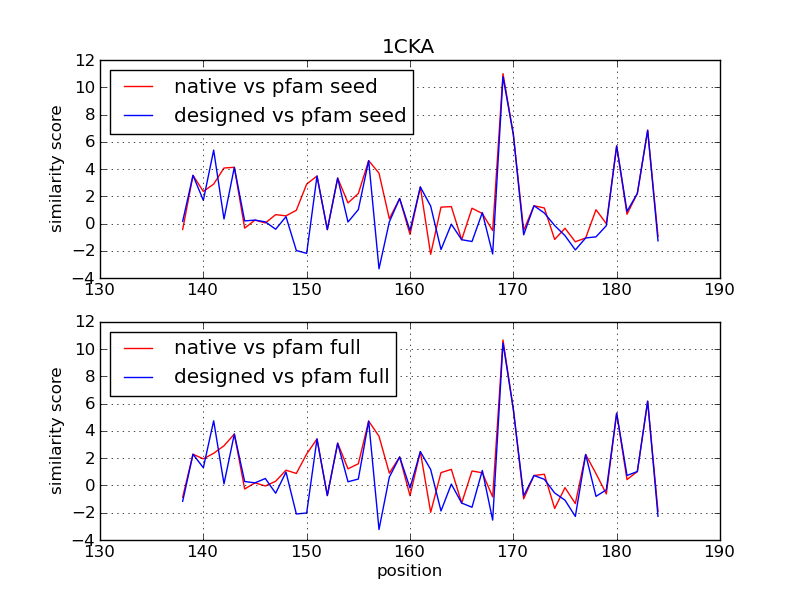
\includegraphics[width=8.45cm]{sedano_gen2/graph_simil_bypos.png} &
       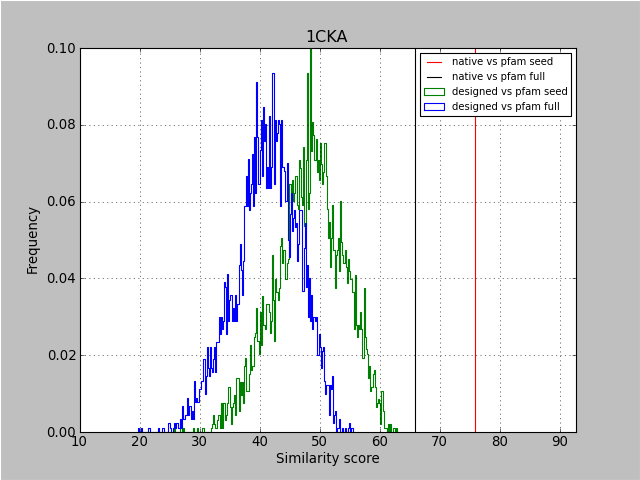
\includegraphics[width=8.45cm]{sedano_gen2/graph_simil_byseq.png} \\


     \end{tabular}

     \caption{Similarité des séquences de 1CKA CORE.}

   \end{figure}


   \begin{figure}[t]
     \centering
     \begin{tabular}{cc}
       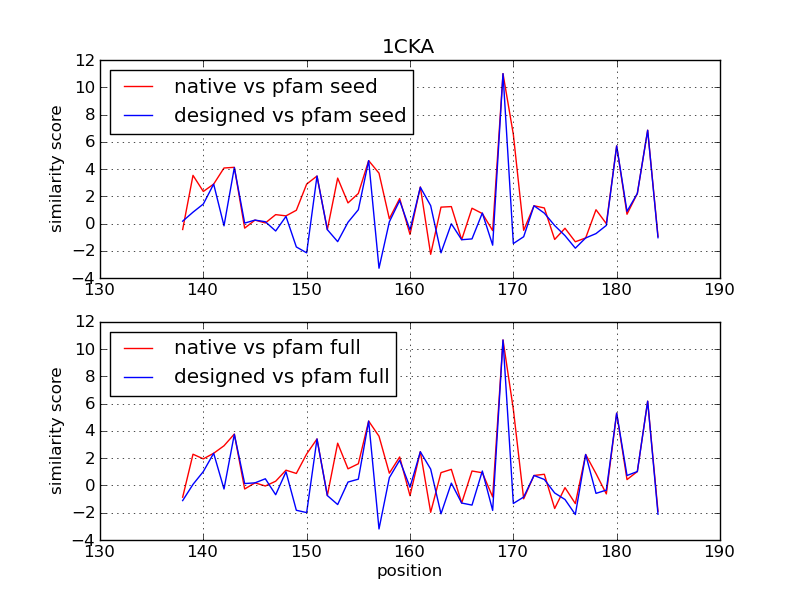
\includegraphics[width=8.45cm]{sedano_gen4/graph_simil_bypos.png} &
       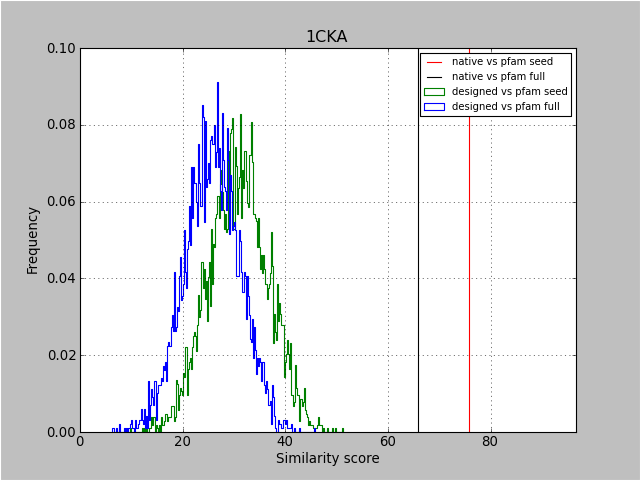
\includegraphics[width=8.45cm]{sedano_gen4/graph_simil_byseq.png} \\

     \end{tabular}

     \caption{Similarité des séquences de 1CKA + LIG.}

   \end{figure}

\end{document}
